\documentclass[]{article}
\usepackage{lmodern}
\usepackage{amssymb,amsmath}
\usepackage{ifxetex,ifluatex}
\usepackage{fixltx2e} % provides \textsubscript
\ifnum 0\ifxetex 1\fi\ifluatex 1\fi=0 % if pdftex
  \usepackage[T1]{fontenc}
  \usepackage[utf8]{inputenc}
\else % if luatex or xelatex
  \ifxetex
    \usepackage{mathspec}
  \else
    \usepackage{fontspec}
  \fi
  \defaultfontfeatures{Ligatures=TeX,Scale=MatchLowercase}
\fi
% use upquote if available, for straight quotes in verbatim environments
\IfFileExists{upquote.sty}{\usepackage{upquote}}{}
% use microtype if available
\IfFileExists{microtype.sty}{%
\usepackage{microtype}
\UseMicrotypeSet[protrusion]{basicmath} % disable protrusion for tt fonts
}{}
\usepackage[margin=1in]{geometry}
\usepackage{hyperref}
\hypersetup{unicode=true,
            pdftitle={The effect of interaction on understanding variable contributions on linear projections},
            pdfauthor={Nicholas Spyrison, Dianne Cook, Kim Marriott},
            pdfkeywords={exploratory data analysis, projection pursuit, high dimensional data,
data visualization, cluster analysis, dimension reduction, statistical
graphics, data science, user study, between users,},
            pdfborder={0 0 0},
            breaklinks=true}
\urlstyle{same}  % don't use monospace font for urls
\usepackage{color}
\usepackage{fancyvrb}
\newcommand{\VerbBar}{|}
\newcommand{\VERB}{\Verb[commandchars=\\\{\}]}
\DefineVerbatimEnvironment{Highlighting}{Verbatim}{commandchars=\\\{\}}
% Add ',fontsize=\small' for more characters per line
\usepackage{framed}
\definecolor{shadecolor}{RGB}{248,248,248}
\newenvironment{Shaded}{\begin{snugshade}}{\end{snugshade}}
\newcommand{\AlertTok}[1]{\textcolor[rgb]{0.94,0.16,0.16}{#1}}
\newcommand{\AnnotationTok}[1]{\textcolor[rgb]{0.56,0.35,0.01}{\textbf{\textit{#1}}}}
\newcommand{\AttributeTok}[1]{\textcolor[rgb]{0.77,0.63,0.00}{#1}}
\newcommand{\BaseNTok}[1]{\textcolor[rgb]{0.00,0.00,0.81}{#1}}
\newcommand{\BuiltInTok}[1]{#1}
\newcommand{\CharTok}[1]{\textcolor[rgb]{0.31,0.60,0.02}{#1}}
\newcommand{\CommentTok}[1]{\textcolor[rgb]{0.56,0.35,0.01}{\textit{#1}}}
\newcommand{\CommentVarTok}[1]{\textcolor[rgb]{0.56,0.35,0.01}{\textbf{\textit{#1}}}}
\newcommand{\ConstantTok}[1]{\textcolor[rgb]{0.00,0.00,0.00}{#1}}
\newcommand{\ControlFlowTok}[1]{\textcolor[rgb]{0.13,0.29,0.53}{\textbf{#1}}}
\newcommand{\DataTypeTok}[1]{\textcolor[rgb]{0.13,0.29,0.53}{#1}}
\newcommand{\DecValTok}[1]{\textcolor[rgb]{0.00,0.00,0.81}{#1}}
\newcommand{\DocumentationTok}[1]{\textcolor[rgb]{0.56,0.35,0.01}{\textbf{\textit{#1}}}}
\newcommand{\ErrorTok}[1]{\textcolor[rgb]{0.64,0.00,0.00}{\textbf{#1}}}
\newcommand{\ExtensionTok}[1]{#1}
\newcommand{\FloatTok}[1]{\textcolor[rgb]{0.00,0.00,0.81}{#1}}
\newcommand{\FunctionTok}[1]{\textcolor[rgb]{0.00,0.00,0.00}{#1}}
\newcommand{\ImportTok}[1]{#1}
\newcommand{\InformationTok}[1]{\textcolor[rgb]{0.56,0.35,0.01}{\textbf{\textit{#1}}}}
\newcommand{\KeywordTok}[1]{\textcolor[rgb]{0.13,0.29,0.53}{\textbf{#1}}}
\newcommand{\NormalTok}[1]{#1}
\newcommand{\OperatorTok}[1]{\textcolor[rgb]{0.81,0.36,0.00}{\textbf{#1}}}
\newcommand{\OtherTok}[1]{\textcolor[rgb]{0.56,0.35,0.01}{#1}}
\newcommand{\PreprocessorTok}[1]{\textcolor[rgb]{0.56,0.35,0.01}{\textit{#1}}}
\newcommand{\RegionMarkerTok}[1]{#1}
\newcommand{\SpecialCharTok}[1]{\textcolor[rgb]{0.00,0.00,0.00}{#1}}
\newcommand{\SpecialStringTok}[1]{\textcolor[rgb]{0.31,0.60,0.02}{#1}}
\newcommand{\StringTok}[1]{\textcolor[rgb]{0.31,0.60,0.02}{#1}}
\newcommand{\VariableTok}[1]{\textcolor[rgb]{0.00,0.00,0.00}{#1}}
\newcommand{\VerbatimStringTok}[1]{\textcolor[rgb]{0.31,0.60,0.02}{#1}}
\newcommand{\WarningTok}[1]{\textcolor[rgb]{0.56,0.35,0.01}{\textbf{\textit{#1}}}}
\usepackage{graphicx,grffile}
\makeatletter
\def\maxwidth{\ifdim\Gin@nat@width>\linewidth\linewidth\else\Gin@nat@width\fi}
\def\maxheight{\ifdim\Gin@nat@height>\textheight\textheight\else\Gin@nat@height\fi}
\makeatother
% Scale images if necessary, so that they will not overflow the page
% margins by default, and it is still possible to overwrite the defaults
% using explicit options in \includegraphics[width, height, ...]{}
\setkeys{Gin}{width=\maxwidth,height=\maxheight,keepaspectratio}
\IfFileExists{parskip.sty}{%
\usepackage{parskip}
}{% else
\setlength{\parindent}{0pt}
\setlength{\parskip}{6pt plus 2pt minus 1pt}
}
\setlength{\emergencystretch}{3em}  % prevent overfull lines
\providecommand{\tightlist}{%
  \setlength{\itemsep}{0pt}\setlength{\parskip}{0pt}}
\setcounter{secnumdepth}{0}
% Redefines (sub)paragraphs to behave more like sections
\ifx\paragraph\undefined\else
\let\oldparagraph\paragraph
\renewcommand{\paragraph}[1]{\oldparagraph{#1}\mbox{}}
\fi
\ifx\subparagraph\undefined\else
\let\oldsubparagraph\subparagraph
\renewcommand{\subparagraph}[1]{\oldsubparagraph{#1}\mbox{}}
\fi

%%% Use protect on footnotes to avoid problems with footnotes in titles
\let\rmarkdownfootnote\footnote%
\def\footnote{\protect\rmarkdownfootnote}

%%% Change title format to be more compact
\usepackage{titling}

% Create subtitle command for use in maketitle
\providecommand{\subtitle}[1]{
  \posttitle{
    \begin{center}\large#1\end{center}
    }
}

\setlength{\droptitle}{-2em}

  \title{The effect of interaction on understanding variable contributions on
linear projections}
    \pretitle{\vspace{\droptitle}\centering\huge}
  \posttitle{\par}
    \author{Nicholas Spyrison, Dianne Cook, Kim Marriott}
    \preauthor{\centering\large\emph}
  \postauthor{\par}
    \date{}
    \predate{}\postdate{}
  

\begin{document}
\maketitle
\begin{abstract}
Principal Component Analysis (PCA) and related eigenvalue techniques are
the traditional standard for viewing prosections of multivariate spaces.
However, the full story of the data is rarely portrayed accurately in a
few projections. More recently, grand tours offer an animation of random
walks offering many angles to view embedded spaces. A manual tour
provides a means of controlling the contribution of individual variables
to a projected subspace. We have developed an application to facilitate
the exploration of multivariate data though the use of various tour
methods. To explore the efficacy of this tool we performed a comparative
user study. Participants in our study performed several high-level
analysis tasks across the three factors and provide subjective ratings.
Accuracy, speed, and qualitative feedback are used to compare and rate
analysts' ability to understand the importance of individual variables'
contribution to distinguishing clustering with the data. User feedback
suggests that\ldots{}
\end{abstract}

\bibliography{spyrison-cook-marriott}

\hypertarget{introduction}{%
\section{Introduction}\label{introduction}}

Multivariate data is ubiquitus in a wide number of fields.

\hypertarget{hypothesis}{%
\section{Hypothesis}\label{hypothesis}}

Does the finer control afforded by the manual tour improve the ability
of the analyst to understand the importance of variables contributing to
the structure?

\hypertarget{sec:design}{%
\section{Experimental design}\label{sec:design}}

\begin{figure}

{\centering 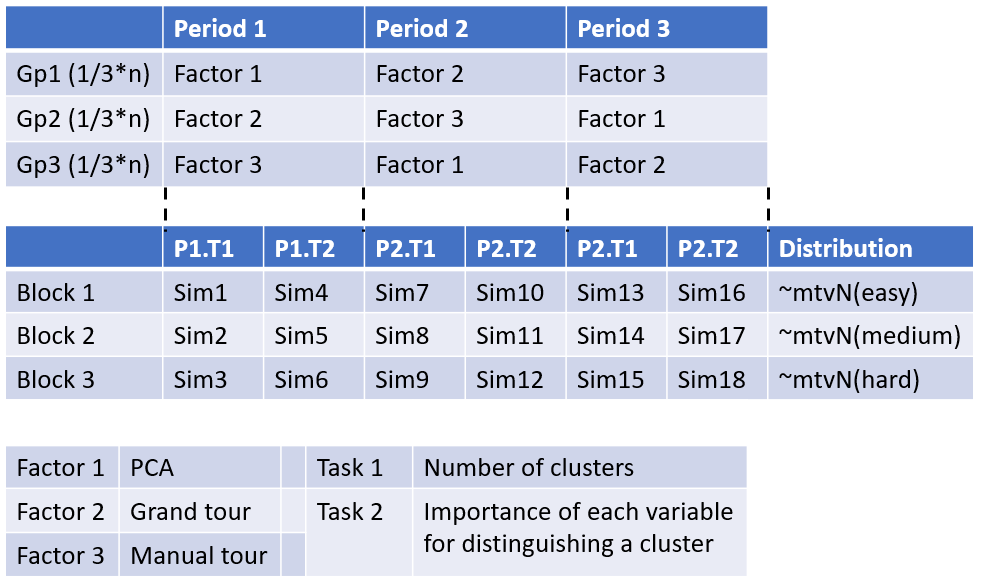
\includegraphics[width=1\linewidth]{./figures/experimental_design} 

}

\caption{Experimental design setup. Participants are assigned to one of 3 even groups controlling the factor order. Within each factor, users perform 3 repetitions of block 1 and then block 2 before proceeding to the next factor. Simulations are used in a fixed order (while factor order changes). Simulations for the first repetition are unique samples drawn from the same distribution. Similarly, the second and third repetitions are drawn from their own more complex distributions.}\label{fig:design}
\end{figure}

\begin{figure}

{\centering 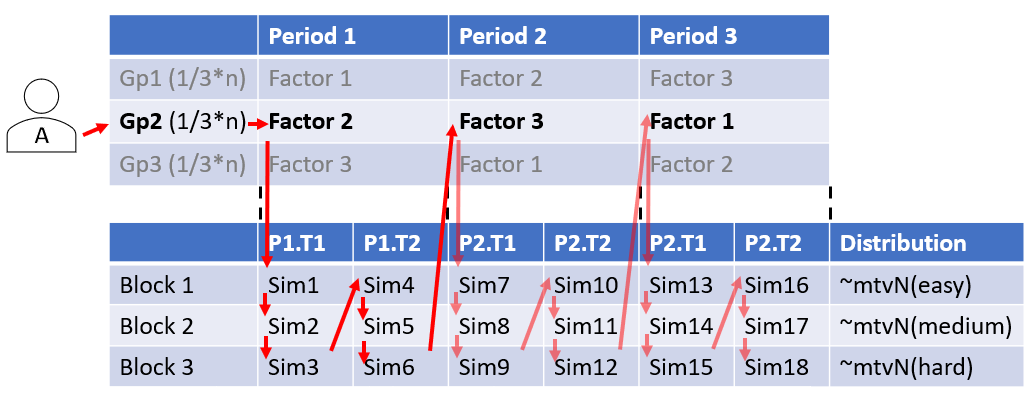
\includegraphics[width=1\linewidth]{./figures/experimental_design_personA} 

}

\caption{Example case. Person `A` is assigned to group 2, where they will use factor 2 (`Grand tour`) for the first period. They perform 3 repetitions of block 1 on simulations of increasing difficulty. Then 3 repetitions of block 2 on unique simulations sampled from the same distributions of increasing difficulty. After this, they proceed to period 2, where they are use factor 3 (`Manual tour`) to perform 3 repetitions of each block. Lastly, in the third period they use factor 1 (`PCA`) to perform the tasks.}\label{fig:designExample}
\end{figure}

\hypertarget{sec:population}{%
\subsection{Participant population}\label{sec:population}}

A sample of convenience was taken from postgraduate students in the
department of econometrics and business statistics and the faculty of
information technology at Monash University, based in Melbourne,
Australia. Participants were required to have prior knowledge of
multivariate data visualizations.

\hypertarget{sec:groups}{%
\subsection{Groups}\label{sec:groups}}

Each participant was randomly split into one of three even factor
groups. The first group was given a biplot -- a scatterplot matrix
coupled with a variable mapping back to original variable space. Users
were allowed to freely choose which two components to view initialized
to PC1 and PC2. The second group was given the same animation, the first
30 seconds of random walk (typically spanning 6 or 7 bases interpolated
into 90 frames viewed at 3 frames per second) of a grand tour with the
ability to freely control the location and speed of the animation. The
third group was provided with the ability to control the magnitude of an
individual variable contributes to the projection with a manual tour.
Doing so performs a constrained rotation on the data object resulting in
a change of the other variables to preserve orthogonality between
dimensions. Participants could freely change which dimension to
manipulate.

\hypertarget{sec:training}{%
\subsection{Training}\label{sec:training}}

\textbf{TODO}

\hypertarget{sec:factors}{%
\subsection{Factors}\label{sec:factors}}

We explored performance across three factors. The first factor is
Principal Component Analysis (\texttt{PCA}). The second factor is an
animated walk of interpolation frames between target bases, called a
\texttt{grand\ tour}. The third factor allows for the manual control of
the individual variable's contribution to the projection, performing a
\texttt{manual\ tour}.

User interface was kept the same whenever possible, but control
interface did change slightly to accomadate differneces between factors.
PCA had two side-by-side radio button selections that control which
prinicipal components were displayed on the x- and y-axes. The manual
tour had same axes selection, with the the addition of a drop-down bar
and slider control. The drop-down selects the variable to manipulate the
contribution of, while the slider controled the magnitude {[}0-1{]} of
the contribution of that variable on the projection. Performing this
manipulation does require the contributions of the other variables to
change if they are to keep their orthogonal relationship.

\hypertarget{sec:blocks}{%
\subsection{Block treatments}\label{sec:blocks}}

Within each factor, participants performed 2 block treatments in a fixed
order. The first block asked participants to identify the number of
clusters present in the data. In this block, clusters were unsupervised,
where all observations appeared as black circles and the basis variable
map was omitted. This block also served as a control for assessing the
general aptitude for this sort of high dimensional analysis as it was
simpler. A second block asked participants to identify any/all variables
that were very important and somewhat important for distinguishing a
given cluster from the others. For instance, which variables are very
important for distinguishing cluster \texttt{b}. This block was
supervised by cluster; observations were assigned shape and (color-blind
friendly) color according to their cluster. A basis variable map was
provided demonstrating the magnitude and direction of the variable
contribution for the given linear projection.

The first block is a ubiquitous task for unsupervised data but was
included as more of a validation task rather than directly addressing
the hypothesis.\\
It was expected that the grand tour should excel in identifying the
number of clusters. This is because the grand tour shows many bases
across all variables viewed in quick succession. This makes for a more
cohesive parallax-like movement between clusters, making them relatively
easy to identify. In contrast, PCA offers the fewest bases with the most
discrete changes. The manual tour explores one dimension at a time. This
exploration views a smaller variable-space than the grand tour,
providing fewer visual cues between clusters.

\hypertarget{sec:reps}{%
\subsection{Repetition}\label{sec:reps}}

Participants were randomly assigned to 1 of 3 even groups. Each group
had a different factor order containing all factors. Both blocks were
performed in the same order. Each block had 3 repetitions performed on
new simulations that were drawn from 3 parameterizations in increasing
difficulty. Each participant went through the simulations in the same
order, while the order of their factor varied. Fixing repetition order
while varying factors should mitigate potential learning bais.

\hypertarget{sec:sim}{%
\subsection{Data simulations}\label{sec:sim}}

The data used for the study were sampled from 4 multivariate normal
distributions. The distributions were parameterized with the number of
clusters, the number of noise variables, and the number of variables.
Each simulation contained either 3 or 4 clusters, with each cluster
containing a random number of observations between 30 and 150. Each
simulation contained 3 or 4 noise variables, which were distributed as
\(~ \mathcal{N}(0, \sigma^2)\). Non-noise variables were distributed
\(~ \mathcal{N}(\mu, \sigma^2)~|~\mu\in \{-3, -2, ... 3\}\). The
variance-covariance matrix was constrained with non-diagonal elements
selected between -0.1 to 0.7, before being constrained into a positive
definitive matrix.

Of the 4 sets of parameterizations, 20 simulations were drawn. The 2
most simple simulations were used during the training section of the
study. All participants were exposed to the same training data sets,
shown in the same order to standardize training. The remaining 18
simulations were drawn such that the remaining 3 parameterizations were
sampled 6 times each. These correspond to the 3 repetitions of a given
factor and block with increasing difficulty. Referring to the middle of
figure \ref{fig:design}, a participant would perform each factor-block
for 3 repetitions with increasing difficultly before proceeding. The
next factor-block has 3 repetitions performed on new simulations but
parameterized for the same order of increasing difficulty. All
participants experience the same order of simulations while varying the
order of the factor (visualization) as controlled by a partition into 3
even groups (top of the same figure).

\hypertarget{sec:response}{%
\subsection{Response \& measures}\label{sec:response}}

Each block was introduced and demonstrated directly preceding each
block. During this introductory segment, each participant was given a
written description of the block task and instructions on how the factor
visualization informed the answer, as illustrated with the same toy data
set. Participants were free to ask questions and clarification from the
proctor at this time. Questions were not allowed outside of the
introductory segments. Participants received exactly \textbf{two}
minutes to explore each repetition's projection before responding to the
given task. Responses came in the form of single integer input for the
block asking to identify the number of clusters. The second block
collected the top 3 ordered variables that distinguish clusters. The
remaining block collected \texttt{p} (number of variables in the data)
inputs grouped into zero to four groups.

After responses for each block were collected, participants were given a
short survey of demographics, related experience, and subjective
evaluation of each factor on a 7-point Likert scale. These questions
covered familiarity and expertise with multivariate data, its
visualization, as well as, ease of use, understandability, confidence,
and likelihood to recommend the participant's factor visualization.

\hypertarget{sec:survey}{%
\subsection{Post-study survey}\label{sec:survey}}

\begin{itemize}
\tightlist
\item
  gender {[}decline, F, M, Intergender/other{]}
\item
  age {[}decline, 19 or younger, 20 to 29, 30 to 39, 40 or older{]}
\item
  completed education {[}decline, highschool, undergraduate,
  honors/masters/mba, doctorate{]}
\item
  experience with data vizualization {[}likert 1-7{]}
\item
  educated in multivarate statistical analysis {[}likert 1-7{]}
\item
  previous familiar with vizualization {[}likert 1-7{]} x3 factors
\item
  ease {[}likert 1-7{]} x3 factors
\item
  confidence {[}likert 1-7{]} x3 factors
\item
  likeability {[}likert 1-7{]} x3 factors 
\end{itemize}

\hypertarget{sec:results}{%
\section{Results}\label{sec:results}}

\hypertarget{sec:spinifex}{%
\section{Accompanying tool: spinifex application}\label{sec:spinifex}}

To accompany this study we have produced a more general use tool to
perform such exploratory analysis of high dimensional data. The
\texttt{spinifex}\{({\textbf{???}})\} R package (version 0.2.0 and up)
contains a free, open-source version of a \texttt{shiny}
\{({\textbf{???}})\} application. The application features traditional
static visualizations including PCA, with biplots and scree plots, and
scatterplot matrices. The application also implements various tours,
including manual tours, projection pursuit, and limited versions of
grand, little, and local tours. Data can be imported in .csv and .rda
format, and projections can be saved as .png, .gif, and .csv formats
where applicable. Run the following R code for help getting started.

\begin{Shaded}
\begin{Highlighting}[]
\KeywordTok{install.packages}\NormalTok{(}\StringTok{"spinifex"}\NormalTok{)}
\NormalTok{spinifex}\OperatorTok{::}\KeywordTok{run_app}\NormalTok{(}\StringTok{"intro"}\NormalTok{)}
\NormalTok{spinifex}\OperatorTok{::}\KeywordTok{run_app}\NormalTok{(}\StringTok{"primary"}\NormalTok{)}
\end{Highlighting}
\end{Shaded}

\hypertarget{sec:discussion}{%
\section{Discussion}\label{sec:discussion}}

\hypertarget{sec:acknowledgments}{%
\section{Acknowledgments}\label{sec:acknowledgments}}

This article was created in R (R Core Team 2019), using
\_CRANpkg\{knitr\} (Xie 2014) and \_CRANpkg\{rmarkdown\} (Xie, Allaire,
and Grolemund 2018), with code generating the examples inline. The
source files for this article be found at
\href{https://github.com/nspyrison/spinifex_paper/}{github.com/nspyrison/spinifex\_study/}.
The source code for the \_pkg\{spinifex\} package and accompanying shiny
application can be found at
\href{https://github.com/nspyrison/spinifex/}{github.com/nspyrison/spinifex/}.

\hypertarget{sec:bib}{%
\section*{Bibliography}\label{sec:bib}}
\addcontentsline{toc}{section}{Bibliography}

\hypertarget{refs}{}
\leavevmode\hypertarget{ref-r_core_team_r:_2019}{}%
R Core Team. 2019. \emph{R: A Language and Environment for Statistical
Computing}. Vienna, Austria: R Foundation for Statistical Computing.
\url{https://www.R-project.org/}.

\leavevmode\hypertarget{ref-stodden_knitr:_2014}{}%
Xie, Yihui. 2014. ``Knitr: A Comprehensive Tool for Reproducible
Research in R.'' In \emph{Implementing Reproducible Computational
Research}, edited by Victoria Stodden, Friedrich Leisch, and Roger D.
Peng. Chapman; Hall/CRC.
\url{http://www.crcpress.com/product/isbn/9781466561595}.

\leavevmode\hypertarget{ref-xie_r_2018}{}%
Xie, Yihui, J. J. Allaire, and Garrett Grolemund. 2018. \emph{R
Markdown: The Definitive Guide}. Boca Raton, Florida: Chapman; Hall/CRC.
\url{https://bookdown.org/yihui/rmarkdown}.


\end{document}
